% !TeX program = xelatex
\documentclass[ebook, oneside]{memoir}

%\overfullrule=2mm

% Colors
\usepackage[svgnames, dvipsnames]{xcolor}
\definecolor{myBlack}{cmyk}{0,0,0,1}
\definecolor{firebrick}{rgb}{0.7, 0.13, 0.13}

% ******************************
%       UTILITIES
% ********************
\input{utilities/arabicwords.tex}
\newcommand{\fatihah}{al-F\={a}ti\d{h}ah}
\newcommand{\baqarah}{al-Baqarah}
\newcommand{\imraan}{\={A}l `Imr\={a}n}
\newcommand{\nisaa}{al-Nis\={a}}
\newcommand{\maidah}{al-M\={a}'idah}
\newcommand{\anaam}{al-An`\={a}m}
\newcommand{\araaf}{al-A`r\={a}f}
\newcommand{\anfaal}{al-Anf\={a}l}
\newcommand{\tawbah}{al-Tawbah}
\newcommand{\yunus}{Y\={u}nus}
\newcommand{\hud}{H\={u}d}
\newcommand{\yusuf}{Y\={u}suf}
\newcommand{\raad}{al-Ra`ad}
\newcommand{\ibrahim}{Ibr\={a}h\={i}m}
\newcommand{\hijr}{al-\d{H}ijr}
\newcommand{\nahl}{al-Na\d{h}l}
\newcommand{\isra}{al-'Isra}
\newcommand{\kahf}{al-Kahf}
\newcommand{\maryam}{Maryam}
\newcommand{\taha}{\d{T}\={a}-H\={a}}
\newcommand{\anbiya}{al-Anbiy\={a}}
\newcommand{\hajj}{al-\d{H}ajj}
\newcommand{\muminoon}{al-Mu'min\={u}n}
\newcommand{\nuur}{al-N\={u}r}
\newcommand{\furqaan}{al-Furq\={a}n}
\newcommand{\shuara}{al-Shu`ar\={a}}
\newcommand{\naml}{al-Naml}
\newcommand{\qasas}{Qa\d{s}a\d{s}}
\newcommand{\ankabut}{al-`Ankab\={u}t}
\newcommand{\ruum}{al-R\={u}m}
\newcommand{\luqman}{Luqm\={a}n}
\newcommand{\sajdah}{al-Sajdah}
\newcommand{\ahzaab}{al-A\date{h}z\={a}b}
\newcommand{\saba}{Saba}
\newcommand{\faatir}{F\={a}\d{t}ir}
\newcommand{\yaseen}{Y\={a} S\={i}n}
\newcommand{\saffaat}{al-\d{S}aff\={a}t}
\newcommand{\sad}{\d{S}\={a}d}
\newcommand{\zumar}{Al-Zumar}
\newcommand{\ghafir}{Gh\={a}fir}
\newcommand{\fussilat}{Fu\d{s}\d{s}ilat}
\newcommand{\shuuraa}{al-Sh\={u}r\={a}}
\newcommand{\zukhruf}{al-Zukhruf}
\newcommand{\dukhaan}{al-Dukh\={a}n}
\newcommand{\jaathiyah}{al-J\={a}thiyah}
\newcommand{\ahqaaf}{al-A\d{h}q\={a}f}
\newcommand{\muhammad}{Mu\d{h}ammad}
\newcommand{\fath}{al-Fat\d{h}}
\newcommand{\hujuraat}{al-\d{H}ujur\={a}t}
\newcommand{\qaf}{Q\={a}f}
\newcommand{\thariyaat}{al-Dhariy\={a}t}
\newcommand{\tuur}{al-\d{T}\={u}r}
\newcommand{\najm}{al-Najm}
\newcommand{\qamr}{al-Qamar}
\newcommand{\rahmaan}{al-Ra\d{h}m\={a}n}
\newcommand{\waqiyah}{al-W\={a}qiyah}
\newcommand{\hadeed}{al-\d{H}ad\={i}d}
\newcommand{\mujaadalah}{al-Muj\={a}dalah}
\newcommand{\hashr}{al-\d{H}ashr}
\newcommand{\mumtahinah}{al-Mumta\d{h}inah}
\newcommand{\saff}{al-\d{S}aff}
\newcommand{\jumuah}{al-Jumu`ah}
\newcommand{\munafiqoon}{al-Mun\={a}fiq\={u}n}
\newcommand{\taghaabun}{al-Tagh\={a}bun}
\newcommand{\talaaq}{al-\d{T}al\={a}q}
\newcommand{\tahreem}{al-Ta\d{h}r\={i}m}
\newcommand{\mulk}{al-Mulk}
\newcommand{\qalam}{al-Qalam}
\newcommand{\haqqah}{al-\d{H}\={a}qqah}
\newcommand{\maarij}{al-Ma`\={a}rij}
\newcommand{\nuh}{Nu\d{h}}
\newcommand{\jinn}{al-Jinn}
\newcommand{\muzzammil}{al-Muzzammil}
\newcommand{\muddathir}{al-Muddathir}
\newcommand{\qiyamah}{al-Qiyamah}
\newcommand{\insaan}{al-Ins\={a}n}
\newcommand{\mursalaat}{al-Mursal\={a}t}
\newcommand{\nabaa}{al-Nab\={a}}
\newcommand{\naziaat}{al-N\={a}zi`\={a}t}
\newcommand{\abasa}{`Abasa}
\newcommand{\takweer}{al-Takw\={i}r}
\newcommand{\infitaar}{al-Infi\d{t}\={a}r}
\newcommand{\mutaffifeen}{al-Mu\d{t}affif\={i}n}
\newcommand{\inshiqaaq}{al-'Inshiq\={a}q}
\newcommand{\burooj}{al-Bur\={u}j}
\newcommand{\tariq}{al-\d{T}\={a}riq}
\newcommand{\alala}{al-A`l\={a}}
\newcommand{\ghashiyah}{al-Gh\={a}shiyah}
\newcommand{\fajr}{al-Fajr}
\newcommand{\balad}{al-Balad}
\newcommand{\shams}{al-Shams}
\newcommand{\lail}{al-Lail}
\newcommand{\duha}{al-\d{D}u\d{h}\={a}}
\newcommand{\shrah}{al-Shra\d{h}}
\newcommand{\tin}{al-T\={i}n}
\newcommand{\alaq}{al-`Alaq}
\newcommand{\qadr}{al-Qadr}
\newcommand{\bayyinah}{al-Bayyinah}
\newcommand{\zalzalah}{al-Zalzalah}
\newcommand{\adiyaat}{al-`\={A}diy\={a}t}
\newcommand{\qariah}{al-Q\={a}ri`ah}
\newcommand{\takathur}{al-Tak\={a}thur}
\newcommand{\asr}{al-`A\d{s}r}
\newcommand{\humazah}{al-Humazah}
\newcommand{\fiil}{al-F\={i}l}
\newcommand{\quraish}{Quraysh}
\newcommand{\maoon}{al-M\={a}`\={u}n}
\newcommand{\kawthar}{al-Kawthar}
\newcommand{\kafiroon}{al-K\={a}fir\={u}n}
\newcommand{\nasr}{al-Na\d{s}r}
\newcommand{\masad}{al-Masad}
\newcommand{\ikhlas}{al-Ikhl\={a}\d{s}}
\newcommand{\falaq}{al-Falaq}
\newcommand{\naas}{al-N\={a}s}

% REFERENCE
  %\newcommand{cmd}{def}
  %\newcommand{}{}

% ******************************
%       MEMOIR SETTINGS
% ********************
\makeheadstyles{default}{%
  \renewcommand*{\secheadstyle}{\color{Maroon}\Large\bfseries}
  \renewcommand*{\subsecheadstyle}{\color{firebrick}\Large\bfseries}
}
\headstyles{default}
\chapterstyle{dowding}

\nouppercaseheads
\makepagestyle{mystyle}
\makeevenhead{mystyle}{}{\textsc{the prophet's prayer}}{\thepage}
\makeoddhead{mystyle}{}{\itshape\leftmark}{\thepage}
\makeevenfoot{mystyle}{}{}{}
\makeoddfoot{mystyle}{}{}{}
\makepsmarks{mystyle}{%
  \createmark{chapter}{left}{nonumber}{}{}
}
\pagestyle{mystyle}

\frenchspacing
\linespread{1.2}

\setlength{\parindent}{10pt}

%\setlength{\parskip}{1em}

    % ******************************
    %       TABLE OF CONTENTS
    % ********************
    \makeatletter
    \renewcommand{\cftchapterleader}{}
    \renewcommand{\cftchapterafterpnum}{\cftparfillskip}
    \renewcommand{\cftchapterpagefont}{}

    % http://tex.stackexchange.com/questions/25694/error-when-trying-to-use-maketextuppercase-to-customize-the-table-of-contents
    \renewcommand*{\l@chapter}[2]{%
      \l@chapapp{\lowercase{#1}}{#2}{\cftchaptername}}
    \renewcommand{\cftchapterfont}{\scshape}

    % 1em space between folio and title
    \renewcommand*{\cftchapterformatpnum}[1]{%
      \cftchapterformatpnumhook{#1}%
      \nolinebreak[4]\hspace*{0.5em}\hbox to \@pnumwidth{{\cftchapterpagefont #1}\hfill}%
    }

    \renewcommand{\cftsectionleader}{}
    \renewcommand{\cftsectionafterpnum}{\cftparfillskip}
    \renewcommand{\cftsectionpagefont}{\color{Maroon}}

    % 1em space between folio and title
    \renewcommand*{\cftsectionformatpnum}[1]{%
      \cftsectionformatpnumhook{#1}%
      \nolinebreak[4]\hspace*{0.5em}\hbox to \@pnumwidth{{\cftsectionpagefont #1}\hfill}%
    }
    \makeatother

% ******************************
%       QURAN AYAH ENV
% ********************
\newcommand{\ayahSize}{0.5}
\def\signed #1{{\leavevmode\unskip\nobreak\hfil\penalty50\hskip2em
    \hbox{}\nobreak\hfil(#1)%
    \parfillskip=0pt \finalhyphendemerits=0 \endgraf}}

\newsavebox\mybox
\newenvironment{aquote}[1]
{\savebox\mybox{#1}\begin{quote}}
  {\signed{\usebox\mybox}\end{quote}}

% ******************************
%       ARABIC ITEM ENV
% ********************
% https://tex.stackexchange.com/questions/355193/list-labels-on-left-with-arabic-using-polyglossia
%\newenvironment{Arabicitem}{\begin{minipage}{\linewidth}\begin{Arabic}}
%    {\end{Arabic}\end{minipage}}

\newenvironment{Arabicitem}{\begin{minipage}[t]{\linewidth}%
    \vspace{-\baselineskip}
    \begin{Arabic}}
    {\end{Arabic}\end{minipage}}

% ******************************
%       NARRATION ENV (APPENDICES)
% ********************
\usepackage[framemethod=default]{mdframed}
\mdfdefinestyle{narration}{%
  topline=false,bottomline=false,rightline=false,%
  linewidth=0.1em,%
  linecolor=Maroon,%
  frametitlealignment=\raggedright%
}

% ******************************
%       PACKAGES
% ********************
%% Start of CMYK Black options
\makeatletter
\newcommand{\globalcolor}[1]{%
  \color{#1}\global\let\default@color\current@color
}
\makeatother

%\AtBeginDocument{\globalcolor{myBlack}}
%% End of CMYK Black options
\usepackage[font=small,skip=2pt]{caption}
\usepackage{xspace}
\usepackage{pdfpages}
\usepackage{minitoc}
\usepackage[protrusion]{microtype}
\usepackage[reset=true, backref=true]{enotez}

    % ******************************
    %       ENOTEZ SETTINGS
    %       http://tex.stackexchange.com/questions/272142/change-color-of-endnotes-markers
    % ********************
    \let\footnote\endnote
    \NewDocumentCommand{\colorendnotemark}{m}{%
      \textsuperscript{\textcolor{Maroon}{#1}}%
    }

    \setenotez{
      mark-cs = \colorendnotemark,
      totoc = section,
      list-name = {Endnotes},
    }

    \DeclareInstance{enotez-list}{normalFont}{list}{
      format = \normalfont,
      list-type = itemize,
    }

\usepackage[%
  hidelinks,
  pdftitle={The Prophet's Prayer},
  pdfauthor={Imām Muḥammad Nāṣir al-Dīn},
  pdfsubject={Religion},
  pdfkeywords={Islam, Religion, Worship, Fiqh, Jurisprudence},
  bookmarksnumbered=true,
  bookmarksopen=false,
  pdfstartview=FitH
]{hyperref}
\usepackage{bookmark}
\usepackage[no-math]{fontspec}
\usepackage{hyphenat}
\usepackage{polyglossia}
\setmainlanguage{english}
\setotherlanguage[numerals=maghrib]{arabic}

% ******************************
%       FONTS
% ********************
\usepackage{realscripts} % Superior fonts - footnote markers
\setmonofont[Scale=0.95]{Inconsolata}
\newfontfamily\arsymbols[
Scale=1.2%
]{KFGQPC Arabic Symbols 01}

\newfontfamily\sakkalfont[
Script=Arabic,%
Scale=1.2%
]{Sakkal Majalla}

\newfontfamily\arabicfont[
Script=Arabic,%
Scale=1.2%,
]{KFGQPC Uthman Taha Naskh}

\newfontfamily\amirifont[Script=Arabic, Scale=0.85]{Amiri}

\newfontfamily\wingdings{Wingdings}
\newcommand\ding[1]{{\wingdings\XeTeXglyph#1}}

\setmainfont[
Numbers=OldStyle,
BoldFont={AGaramondPro-Bold.otf},
ItalicFont={AGaramondPro-Italic.otf},
BoldItalicFont={AGaramondPro-BoldItalic.otf},
SmallCapsFont={AGaramondPro-Regular.otf},
SmallCapsFeatures={Letters=SmallCaps},
UprightFeatures = { SizeFeatures= {
    {Size=-10, OpticalSize=8 },
    {Size= 10-14, OpticalSize=10},
    {Size= 14-18, OpticalSize=14},
    {Size= 18-, OpticalSize=18}}}
]{AGaramondPro-Regular.otf}

%\XeTeXinterchartokenstate=1
\newXeTeXintercharclass\confb % connect back
\newXeTeXintercharclass\conb  % connect front back
\newXeTeXintercharclass\alif  % alif
\newXeTeXintercharclass\lam   % lam
%\newXeTeXintercharclass\ha   % ha

\XeTeXcharclass `\ي=\confb 
\XeTeXcharclass `\ئ=\confb
\XeTeXcharclass `\ه=\confb
\XeTeXcharclass `\ش=\confb
\XeTeXcharclass `\س=\confb
\XeTeXcharclass `\ق=\confb
\XeTeXcharclass `\ف=\confb
\XeTeXcharclass `\غ=\confb
\XeTeXcharclass `\ع=\confb
\XeTeXcharclass `\ض=\confb
\XeTeXcharclass `\ص=\confb
\XeTeXcharclass `\ن=\confb
\XeTeXcharclass `\م=\confb
\XeTeXcharclass `\ك=\confb
\XeTeXcharclass `\ظ=\confb
\XeTeXcharclass `\ط=\confb
\XeTeXcharclass `\خ=\confb
\XeTeXcharclass `\ح=\confb
\XeTeXcharclass `\ج=\confb
\XeTeXcharclass `\ث=\confb
\XeTeXcharclass `\ت=\confb
\XeTeXcharclass `\ب=\confb

\XeTeXcharclass `\ل=\lam

\XeTeXcharclass `\ا=\alif
\XeTeXcharclass `\أ=\alif
\XeTeXcharclass `\إ=\alif
\XeTeXcharclass `\آ=\alif

%\XeTeXcharclass `\ه=\ha

\XeTeXcharclass `\و=\conb
\XeTeXcharclass `\ؤ=\conb
\XeTeXcharclass `\ذ=\conb
\XeTeXcharclass `\د=\conb
\XeTeXcharclass `\ز=\conb
\XeTeXcharclass `\ر=\conb
\XeTeXcharclass `\ة=\conb

\XeTeXinterchartoks \confb \confb = {\kashida{}}
\XeTeXinterchartoks \lam \lam     = {\kashida{}}
\XeTeXinterchartoks \confb \alif  = {\kashida{}}
\XeTeXinterchartoks \confb \lam   = {\kashida{}}
\XeTeXinterchartoks \lam \confb   = {\kashida{}}
\XeTeXinterchartoks \lam \conb    = {\kashida{}}
\XeTeXinterchartoks \confb \conb  = {\kashida{}}
%\XeTeXinterchartoks \alif \lam \lam \ha = = {\kashida{}}

\newlength\kashidaheight
\setlength\kashidaheight{\heightof{\textarabic{ـ}}} \newlength\kashidadepth
\setlength\kashidadepth{\depthof{\textarabic{ـ}}}

\newcommand\kashida[1]{\char"200D
        \nobreak\leaders
        \hrule height \kashidaheight depth \kashidadepth
        \hskip 0pt plus 100 pt
        \nobreak\char"200D}

\newcommand{\pbuh}{{\color{Goldenrod}\sakkalfont{\symbol{"FDFA}}}\xspace}
\newcommand{\mabpwhim}{{\arsymbols{\XeTeXglyph 73}}\xspace}
\newcommand{\mabpwher}{{\arsymbols{\XeTeXglyph 74}}\xspace}
\newcommand{\mabpwthemtwo}{{\arsymbols{\XeTeXglyph 76}}\xspace}
\newcommand{\mabpwthem}{{\arsymbols{\XeTeXglyph 75}}\xspace}
\newcommand{\mabpwthemf}{{\arsymbols{\XeTeXglyph 77}}\xspace}
\newcommand{\ohsalam}{{\arsymbols{\XeTeXglyph 79}}\xspace}

% ******************************
%       HYPHENATION
% ********************
\hyphenation{%
con-curred
whe-ther
refuta-tion
breth-ren
aḥā-dīth
madhā-hib
muqalli-dīn
Taḥ-dhīru-hum
Takh-rīj
Ṣugh-rā
manu-script
istirā-ḥah
pro-phets
Pro-phet
Ṭal-ḥah
Muḥam-mad
maw-qūf
Ibrā-hīm
Qu-ran
ikh-ti-lāf
Raḥ-mān
}

\begin{document}
\cleardoublepage
\pdfbookmark{Cover}{Cover}
\includepdf[fitpaper]{cover/cover}

\includepdf[fitpaper]{bismillah-page}

%\includepdf{preview-release-note}

\pdfbookmark[0]{Transliteration Key}{TransliterationKey}
\includepdf{transliteration_key}

% ******************************
\frontmatter
% ********************
\pdfbookmark{\contentsname}{Contents}
\dominitoc
\tableofcontents*

\include{permission}

%\input{preface}
%\cleardoublepage

\input{editors-note}
\cleardoublepage

%\input{acknowledgements}
%\cleardoublepage

\input{author-biography}
\cleardoublepage

\input{fm1}
\cleardoublepage
\printendnotes[normalFont]

\input{fm2}
\cleardoublepage
\printendnotes[normalFont]

% ******************************
\mainmatter
% ********************
\input{chapter1} % Facing the Ka'bah
\cleardoublepage
\printendnotes[normalFont]
\input{chapter2} % Standing in Prayer
\cleardoublepage
\printendnotes[normalFont]
\input{chapter3} % Intention and Takbir
\cleardoublepage
\printendnotes[normalFont]
\input{chapter4} % Opening Supplications
\cleardoublepage
\printendnotes[normalFont]
\input{chapter5} % Recitation
\cleardoublepage
\printendnotes[normalFont]
\input{chapter6} % The Ruku
\cleardoublepage
\printendnotes[normalFont]
\input{chapter7} % The Sujud
\cleardoublepage
\printendnotes[normalFont]
\input{chapter8} % The Second Rakah
\cleardoublepage
\printendnotes[normalFont]
\input{chapter9} % The First Tashahhud
\cleardoublepage
\printendnotes[normalFont]
\input{chapter10} % The Last Tashahhud
\cleardoublepage
\printendnotes[normalFont]
\input{chapter11} % The Taslim
\cleardoublepage
\printendnotes[normalFont]

\addtocontents{toc}{%
  \protect \newpage
  \protect \bigskip\noindent
  \protect \centering
  \protect \Large{%
  \protect\textsc{--- appendices ---}}\par%
}

\begin{appendices}
\input{appendix1} %
\input{appendix2} %
\input{appendix3} %
\input{appendix4} %
\input{appendix5} %
\hypertarget{analysis-of-the-narrations-regarding-the-saying-of-ux101mux12bn-by-the-imam-and-the-congregation}{%
\chapter{Analysis of the narrations regarding the saying of āmīn by the
Imam and the
Congregation}\label{analysis-of-the-narrations-regarding-the-saying-of-ux101mux12bn-by-the-imam-and-the-congregation}}

\chaptermark{The saying of āmīn by the Imam and the Congregation}

From: \emph{Silsilah al-Aḥādīth al-Ḍaʿīfah} (\#951--\#952) by Shaykh
al-Albānī.

\begin{mdframed}[style=narration, frametitle={Narration \#951}]
When he said \textit{āmīn}, those behind him would say \textit{āmīn}, such that there was a lot of noise in the mosque.
\end{mdframed}

There is \textsc{no basis} for the \emph{ḥadīth} with this wording as
far as we know. Ibn Ḥajr said in \emph{al-Talkhīṣ al-Ḥabīr} (p.~90), ``I
do not find it with this wording, but its meaning is related by Ibn
Mājah in the \emph{ḥadīth} of Bishr bin Rāfiʿ (i.e. \textit{ḥadīth} \#952).'' He then said,

\begin{quote}
\textcolor{MidnightBlue}{Ibn Ṣalāh said in his book
\emph{al-Wasīṭ} that al-Ghazzālī narrated this \emph{ḥadīth} like this
in the same manner as Imam al-Ḥaramayn, as he ultimately narrated it
like this, and it is not \emph{ṣaḥīḥ}, albeit \emph{marfūʿ}. Imam
al-Shāfiʿī narrated this \emph{ḥadīth} from ʿAṭā and said, “I used to
hear Imam Ibn Zubayr and those after him say \emph{āmin} until the
mosque trembled.” Imam al-Nawawī said something similar as if he and Ibn
Ṣalāh wanted this wording of the \emph{ḥadīth}. However, the context
provided by Ibn Mājah provides some meanings we produced earlier.}
\end{quote}

\textcolor{MidnightBlue}{The aforementioned
indicates that the context of Ibn Mājah provides the entirety of the
meaning, not part of it. If it is pondered on, the context cited above
contains either some of the meaning or all of it. As for some of the
meaning, this means that the Imam is the only one audible, as for the
entirety of the meaning, this means that those being led in prayer are
also audible, as is highlighted in the \emph{ḥadīth}, ``\ldots and the
mosque would shake with it.'' The \emph{ḥadīth} indicates that the
loudness of their voices is the reason the masjid shook, and this is
probable, and this is the wording of Ibn Mājah.}

\begin{mdframed}[style=narration, frametitle={Narration \#952}]
When he recited “Not of those who received Your anger, nor of those who go astray,” he said \textit{āmīn}, such that those close to him in the first row could hear (and the mosque trembled with it).
\end{mdframed}

\emph{Ḍaʿīf} (\textsc{Weak}). Related by Ibn Mājah (1/281) and Abū Dāwūd
without the addition (1/148), both via:

Bishr bin Rāfiʿ from Abū ʿAbd Allāh, son of the maternal uncle of (i.e. cousin of) Abū Hurayrah \mabpwhim,
from Abū Hurayrah \mabpwhim from the Prophet \pbuh.

\textcolor{MidnightBlue}{This chain is weak. Al-Ḥafiẓ
al-Zarʿah ibn al-ʿIraqī's saying, ``Its chain is good,'' is not good and will be clarified with the proceeding statements.}
%It makes clear what is brought forward from the \emph{ḥadīth}.}

Ibn Ḥajar said in \emph{al-Talkhīṣ} (p.~90), ``Bishr bin Rāfiʿ is weak;
the cousin of Abū Hurayrah \mabpwhim has been said to be unknown, but
Ibn Ḥibbān has declared him reliable.''

Al-Būṣayrī said in \emph{al-Zawāʾid} (56/1), ``This is a weak
\emph{isnād}; Abū ʿAbd Allāh's condition is not known; Bishr was
declared weak by Aḥmad, and Ibn Ḥibbān said, `He narrated
fabrications.'\,''

\textcolor{MidnightBlue}{What Ibn Ḥibbān said
is good (179:1): ``As if it were intentional.'' It is among the
speculations of al-Shawkānī, may Allah have mercy on him; he said about
this\emph{ḥadīth}---after it was mentioned by Majd ibn Taymīyyah with the
wording of Abū Dāwūd and the wording of Ibn Mājah (188/2)---that ``This \emph{ḥadīth} was also taken from al-Dāraquṭnī, and he
said, `Its chain is \emph{ḥasan},' and al-Ḥākim said, `It is
\emph{ṣaḥīḥ} according to their two conditions.' Al-Bayhaqī said, `It is
\emph{ḥasan ṣaḥīḥ}.'\,''. These scholars used the following wording in
their narrations, ``When he \pbuh finished reciting \emph{Umm al-Qurʾān}
he would raise his voice and say: \emph{Āmin}.'' It is not mentioned any
recital from the row or otherwise. This wording does not contain the
wording found in Ibn Mājah, which relates that those being led in prayer
would say \emph{Āmin} so loudly that the mosque would shake. This
confirms the difference between the two narrations, and it is not
permissible to ascribe to the first except to the exclusion of the
second, and this is apparent. The wording in this narration is also
weak. Among the narrators is Isḥāq bin Ibrāhīm bin al-ʿAlā al-Zubīd, and
he is more commonly known as Ibn Zabrīq, and he is weak. Abū Ḥātim said,
``There is no problem with him.'' And Ibn Maʿīn praised him. Al-Nasāʾī
said, ``He is not trustworthy.'' Muḥammad bin ʿAwf said, ``I doubt that
Isḥaq bin Zabrīq used to lie.''}

\textcolor{MidnightBlue}{(MISSING SENTENCE)\ldots{}in
his \emph{Musnad} (76/1): ``The \emph{ḥadīth} was taken from Muslim bin
Khālid from Ibn Jurayj from ʿAṭā, he said: ``I used to hear the Imams,
and Ibn al-Zubayr mentioned, and those after him, say \emph{Āmin}, and
those behind the Imams used to say \emph{Āmin} loudly in the masjid.''
Al-Ḥāfiẓ was quiet on the issue as was mentioned previously, there are
two reasons for this: The first, the weakness of Muslim bin Khālid, also
known as al-Zinjī. (MISSING SENTENCE)}

\textcolor{MidnightBlue}{(MISSING SENTENCE) The
second, is that Ibn Jurayj was a cheat. Perhaps he received it from the
maternal uncle of Ibn Abī Anūf from ʿAṭā with the wording: ``I witnessed
two Companions of the Messenger of Allāh \pbuh in the Masjid (al-Ḥarām),
when the Imam recites, `and those who go astray,' those who were being
led in prayer raised their voices and said \emph{Āmin},'' (in another
narration) ``I heard the tremor from their \emph{Āmin}.'' Taken from Ibn
Mājah's \emph{al-Thuqāt} (2:74) and al-Bayhaqī (2:59) who also has
another narration (MISSING SENTENCE) and he did not mention the
\emph{jarḥ} and \emph{taʿdīl}. Ibn Ḥibban narrates it in
\emph{al-Thuqāt}, and he imparts this (MISSING SENTENCE) For this
reason, I am not convinced by it strength (MISSING SENTENCE) It is also
apparent that Imam al-Shāfiʿī was not convinced by the strength of the
narration. He said in \emph{al-Umm} (95/1): ``If the Imam finishes
reciting \emph{Umm al-Qurʾān} and says \emph{Āmin} and raises his voice,
those praying behind him imitate him, if the Imam says it, then they say
it, and they hear themselves, and I don't like that they say it out
loud.'' This statement is confirmed by the companions of Imam al-Shāfiʿī
that he did not like it, thus, the most correct opinion regarding this
issue is that which Imam al-Shāfiʿī opted for, which is that the Imam
recites loudly and those behind him do not. And Allāh knows best.}

This \emph{ḥadīth} only gives a part of the meaning of the one before
it, i.e.~the saying of \emph{āmīn} by the Imam alone. As for the
\emph{āmīn} of those behind, this could be the reason for the phrase
``the mosque trembled with it (the sound),'' but the \emph{ḥadīth}
literally implies that the \emph{āmīn} of the Prophet \pbuh was the
reason for this.

\begin{mdframed}[style=narration, frametitle={Narration}]
When he finished reciting the Mother of the Quran, he raised his voice and said \textit{āmīn}.
\end{mdframed}

\emph{Ḍaʿīf} (\textsc{Weak}). Related by al-Dāraquṭnī, al-Ḥākim, and
al-Bayhaqī.

All the above sources contain Isḥāq bin Ibrāhīm bin al-ʿAlā al-Zubaydī,
also known as Ibn Zibrīq, who is weak: Abū Ḥātim said, ``An old man, no
harm in him;'' Ibn Maʿīn described him in good terms; al-Nasāʾī said,
``Not reliable;'' Muḥammad bin ʿAwf said, ``I have no doubt that Isḥāq
bin Zibrīq used to lie.'' However, this wording is correct in meaning,
for it has a supporting \emph{ḥadīth} of Wāʾil bin Ḥajar with a
\emph{ṣaḥīḥ sanad}.

(Since the text of this \emph{ḥadīth} does not imply the \emph{āmīn} of
the congregation at all, it is incorrect to regard it as another version
of \emph{ḥadīth} no. 2, as al-Shawkānī did.)

The only support for no. 1 is what al-Shāfiʿī related in his
\emph{Musnad} (1/76) via Muslim bin Khālid from Ibn Jurayj from ʿAtā,
who said:

\begin{mdframed}[style=narration, frametitle={Narration}]
I used to hear the Imams: Ibn al-Zubayr and others after him would say \textit{āmīn}, and those behind would say \textit{āmīn}, until the mosque echoed.
\end{mdframed}

This has two defects:

\begin{enumerate}
\def\labelenumi{\roman{enumi}.}
\tightlist
\item
  The weakness of Muslim bin Khālid al-Zanjī; Ibn Ḥajar said, ``He was
  truthful, but made many errors.''
\item
  The \emph{ʿanʿanah} of Ibn Jurayj, who was a \emph{mudallis}; perhaps
  he actually took it from Khālid bin Abī Anūf, who narrated it from
  ʿAtā as follows:
\end{enumerate}

\begin{mdframed}[style=narration, frametitle={Narration}]
I came across two hundred Companions of the Messenger of Allāh \pbuh in this mosque (i.e. Masjid al-Ḥarām, Makkah): when the Imam had said “Nor of those who go astray,” they raised their voices in \textit{āmīn} (in one narration: I heard the thundering sound of their \textit{āmīn}).
\end{mdframed}

Related by al-Bayhaqī (2/59) and Ibn Ḥibbān in \emph{al-Thiqāt} (2/74);
the alternative narration is from the former.

This Khālid was described by Ibn Abī Ḥātim (1/2/355--366), but he did
not include any authentication or disparagement. Ibn Ḥibbān included him
among the reliable narrators, but Ibn Ḥibbān is well-known to be far
from rigorous in such cases, so I am not satisfied that this narration
is authentic. This is because if Ibn Jurayj indeed took it from him,
this constitutes only one debatable route; if not, we do not know from
whom Ibn Jurayj took it. It seems that Imam al-Shāfiʿī himself was not
satisfied of the authenticity of this narration, for his position is
contrary to it: he says in \emph{al-Umm} (1/95), ``So when the Imam
completes reciting the Mother of the Book, he says \emph{āmīn}, raising
his voice so that those behind may follow him: when he says it, they say
it to themselves, but I do not like them saying it aloud;'' Had the
above narration from the Companions been authentic in al-Shāfiʿī's view,
he would not have opposed their action.

Hence, the most correct opinion in this issue appears to be the
\emph{madhhab} of al-Shāfiʿī: that the Imam, but not those following,
should say \emph{āmīn} loudly. Allāh knows best.

But then, I saw that al-Bukhārī mentioned the text (only) of the
narration about Ibn al-Zubayr in his \emph{Ṣaḥīḥ} (i.e.~in
\emph{muʿallaq} form), designating it with certainty. Ibn Ḥajar said in
\emph{Fatḥ al-Bārī} (2/208), ``The connecting \emph{isnād} has been
provided by ʿAbd al-Razzāq from Ibn Jurayj from ʿAtā. He (i.e.~Ibn
Jurayj) said, `I said to him, ``Did Ibn al-Zubayr say \emph{āmīn} at the
end of the Mother of the Quran?'' He said, ``Yes, and those behind him
also said \emph{āmīn}, until the mosque echoed.'' He then said,
``Verily, \emph{āmīn} is a supplication.''\,'\,'' This is found in the
\emph{Muṣannaf} of ʿAbd al-Razzāq (2640/2), and from this route, in Ibn
Ḥazm's \emph{al-Muḥallā} (3/364).

In this narration, Ibn Jurayj has clarified that he took the narration
from ʿAtā face-to-face, so we are assured of the absence of
\emph{tadlīs}, and the narration of Ibn al-Zubayr is established firmly.
Similarly is proven from Abū Hurayrah \mabpwhim; Abū Rāfī said:

\begin{mdframed}[style=narration, frametitle={Narration}]
Abū Hurayrah used to call to prayer for Marwān bin al-Ḥakam, stipulating that the latter would not get to “Nor of those who go astray” unless he knew that Abū Hurayrah had entered the row. So when Marwān said “Nor of those who go astray,” Abū Hurayrah would say \textit{āmīn}, prolonging it. He also said, “When the \textit{āmīn} of those on the earth coincides with the \textit{āmīn} of those in the heaven, they are forgiven.”
\end{mdframed}

Related by al-Bayhaqī (2/59); its \emph{isnād} is \emph{ṣaḥīḥ}.

Hence, since nothing is established from any of the Companions other
than Abū Hurayrah and Ibn al-Zubayr \mabpwthem contrary to their
\emph{āmīn} \textsc{aloud}, this must be accepted. Presently, I know of
no narration opposing this. Allāh knows best.
 %
\input{appendix7} %
\input{appendix8} %
\hypertarget{four-places-of-prayer-haram}{%
  \chapter{Four places of prayer in Masjid al-Ḥarām}\label{four-places-of-prayer-haram}}

\chaptermark{Four places of prayer in Masjid al-Ḥarām}

The following is an excerpt (pp.\ 109–10) from \textit{The Story of a Pilgrimage to Hijaz} (Calcutta: Thacker, Spink \& Co, 1909) by Her Highness, the Nawab Sultan Jahan Begum (i.e. Sultan Kaikhusrau Jahan Begum), Ruler of Bhopal (1858--1930).\\
\hrule

\begin{figure}
  \begin{center}
    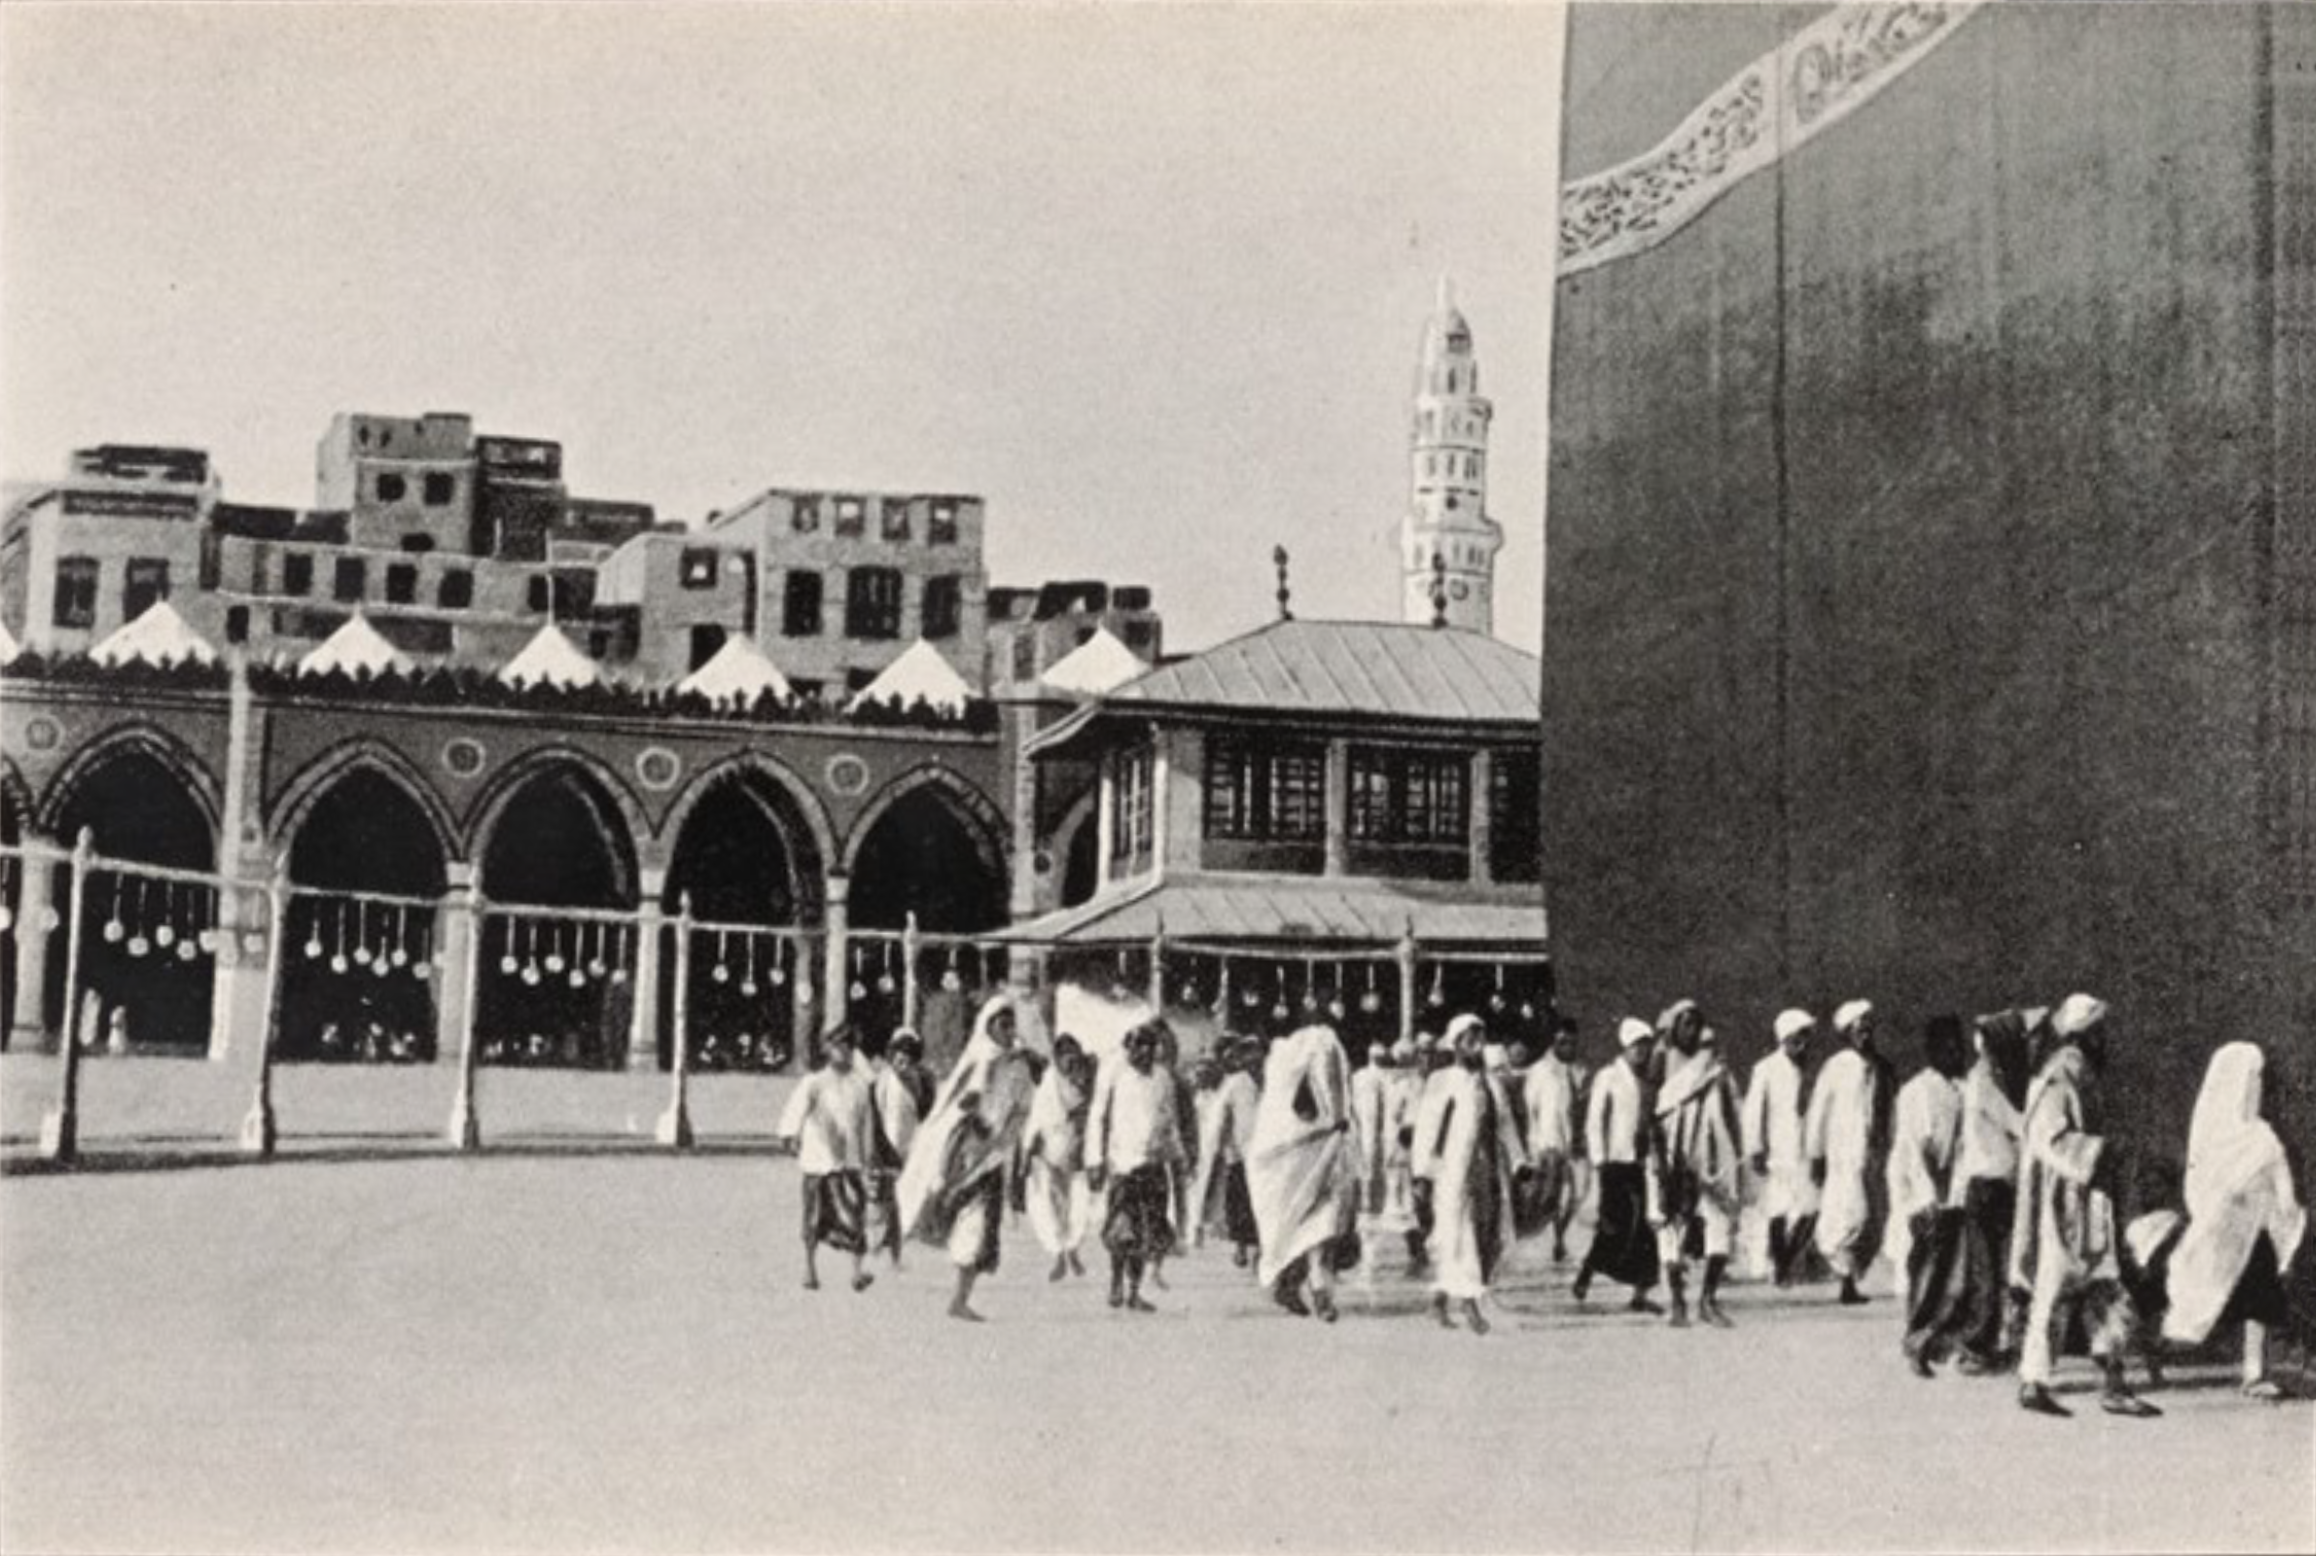
\includegraphics[width=0.84\textwidth]{images/haram2}
  \end{center}
  \caption*{Muṣallā Ḥanafī (p.\ 109).}
\end{figure}

\section*{Maqām Muṣallā Ḥanafī}

Inside the Ḥarām is a Muṣallā (place of prayer) surmounted by two brass spires where the Imam of the Ḥanafīs prays with those of his sect. The majority of the inhabitants of India and Turkistan are Ḥanafīs.

\section*{Maqām Muṣallā Shāfiʿī}

This Muṣallā, which stands close to the well of Zamzam, has a single brass spire. It is set apart for the worship of the Shāfiʿīs, the sect to which most Arabs belong.

\section*{Maqām Muṣallā Mālikī}

At this Muṣallā, which has one brass spire, the Imam of te Mālikīs stands to pray. The people of the Western countries are for the most parts[\textit{sic}] Mālikīs.

\section*{Maqām Muṣallā Ḥanbalī}

The Ḥanbalīs' Muṣallā has one brass spire. Most Arabs are followers of the Ḥanbalī school. The four Muṣallās above belong to the Sunnīs; The Shīʿas and the Khārijīs have no concern with them.

\begin{figure}[ht]
  \begin{center}
    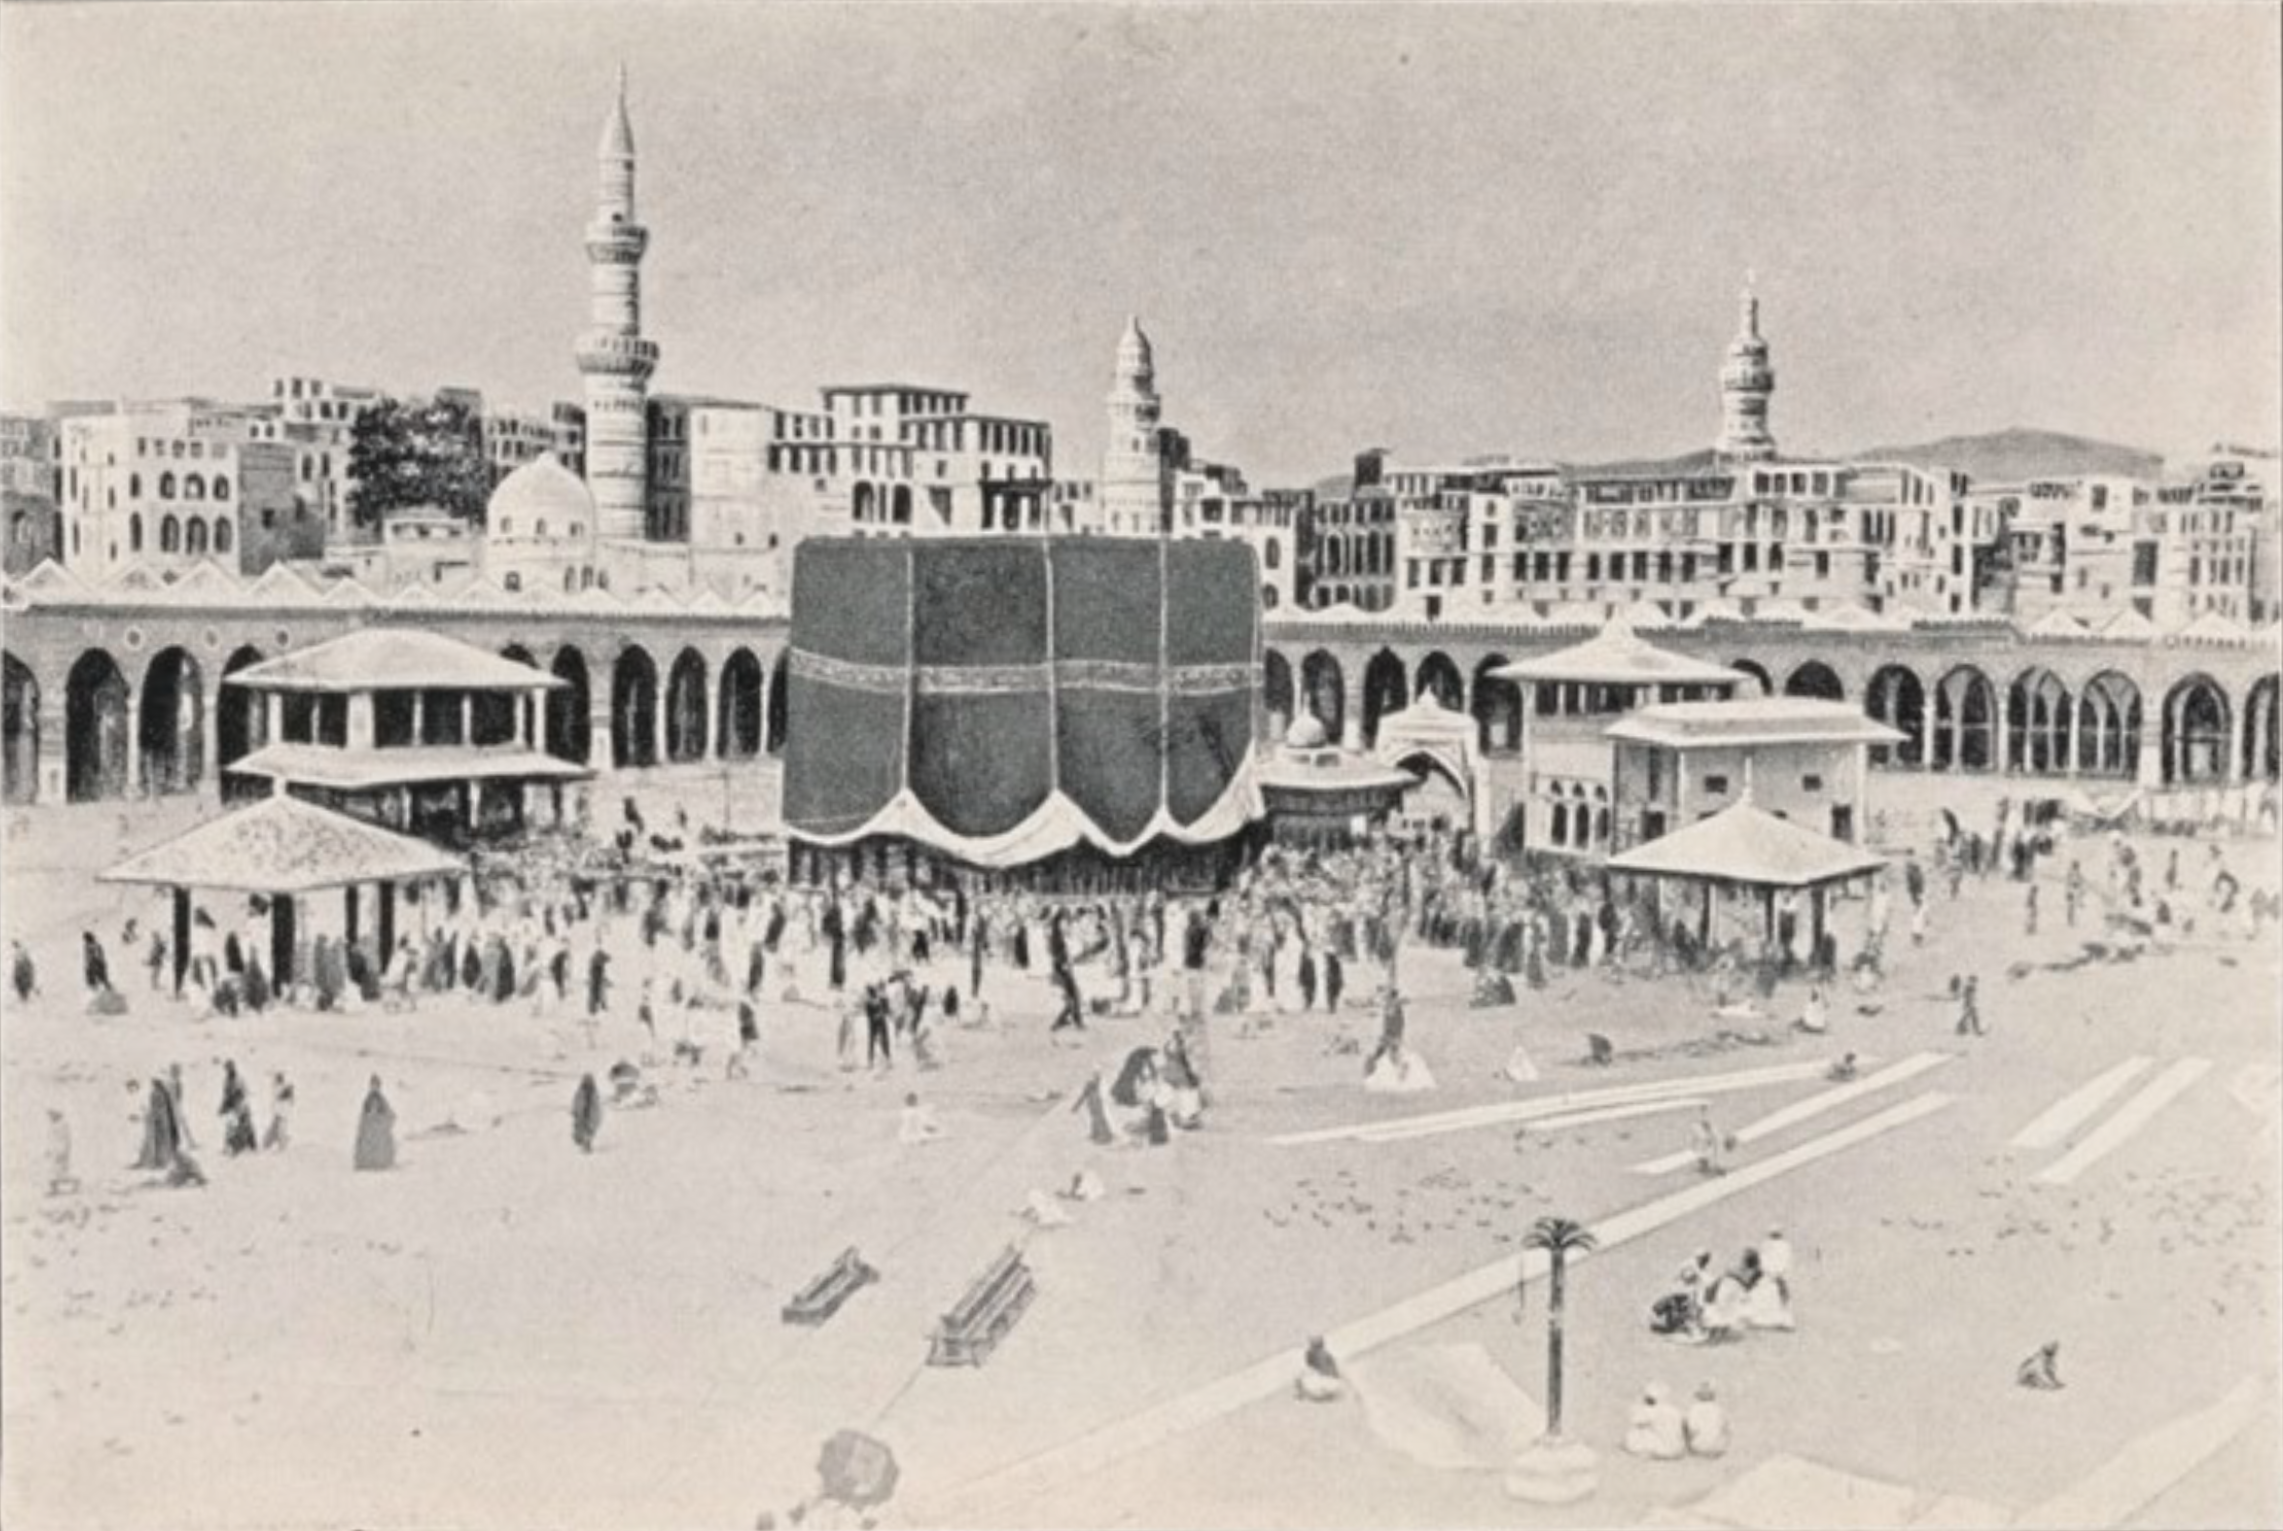
\includegraphics[width=0.84\textwidth]{images/haram1}
  \end{center}
  \caption*{Masjid al-Ḥarām al-Sharīf (p.\ 44).}
\end{figure} %
\input{addendum} %
\end{appendices}

% ******************************
\backmatter
% ********************
\pdfbookmark[0]{Quran Chapter List}{QuranChapterList}
\includepdf[pages={1-}]{_quran_chapter_list}
\end{document}